\documentclass[aspectratio=169,11pt]{beamer}

% -----------------------------------------------------------------------------
% Self-contained style: this deck no longer depends on a missing style.tex file.
% -----------------------------------------------------------------------------
\usepackage[T1]{fontenc}
\usepackage{lmodern}
\usepackage{amsmath,amssymb,mathtools}
\usepackage{booktabs}
\usepackage{tabularx}
\usepackage{listings}
\usepackage{tikz}
\usepackage[most]{tcolorbox}
\usepackage{appendixnumberbeamer}
\usetikzlibrary{arrows.meta,calc,fit,matrix,positioning,shapes.geometric}

\usetheme{Boadilla}
\usecolortheme{seagull}
\setbeamertemplate{navigation symbols}{}
\setbeamertemplate{items}[circle]
\setbeamertemplate{enumerate items}[default]
\setbeameroption{hide notes} % Use show notes or show notes on second screen when teaching.

\definecolor{osblue}{RGB}{28,86,145}
\definecolor{osgreen}{RGB}{36,125,91}
\definecolor{osorange}{RGB}{202,105,36}
\definecolor{osred}{RGB}{166,45,45}
\definecolor{osgray}{RGB}{74,85,104}
\setbeamercolor{structure}{fg=osblue}
\setbeamercolor{alerted text}{fg=osred}
\setbeamercolor{block title}{bg=osblue!15,fg=black}
\setbeamercolor{block body}{bg=osblue!4,fg=black}

\newcommand{\concept}[1]{\textcolor{osblue}{\textbf{#1}}}
\newcommand{\code}[1]{\texttt{#1}}
\newcommand{\smallnote}[1]{\par\vspace{0.2em}{\scriptsize\color{osgray}#1}}

\tcbset{
  enhanced,
  boxrule=.7pt,
  arc=1.5mm,
  left=1.2mm,right=1.2mm,top=.8mm,bottom=.8mm,
  colback=osblue!3,
  colframe=osblue!60
}

\lstset{
  basicstyle=\scriptsize\ttfamily,
  keywordstyle=\color{osblue}\bfseries,
  commentstyle=\color{osgreen!80!black},
  stringstyle=\color{osred},
  numbers=left,
  numberstyle=\tiny\color{osgray},
  numbersep=5pt,
  frame=single,
  rulecolor=\color{black!20},
  backgroundcolor=\color{black!2},
  breaklines=true,
  showstringspaces=false,
  columns=fullflexible,
  keepspaces=true
}

\setbeamertemplate{footline}{%
  \leavevmode%
  \hbox{%
    \begin{beamercolorbox}[wd=.18\paperwidth,ht=2.6ex,dp=1.1ex,center]{author in head/foot}
      \insertshortauthor
    \end{beamercolorbox}%
    \begin{beamercolorbox}[wd=.64\paperwidth,ht=2.6ex,dp=1.1ex,center]{title in head/foot}
      \insertshorttitle\ifx\insertsection\empty\else\enspace---\enspace\insertsection\fi
    \end{beamercolorbox}%
    \begin{beamercolorbox}[wd=.18\paperwidth,ht=2.6ex,dp=1.1ex,center]{date in head/foot}
      \insertframenumber{} / \inserttotalframenumber
    \end{beamercolorbox}%
  }
}

\AtBeginSection[]{
  \begin{frame}[plain,noframenumbering]{Road map}
    \tableofcontents[currentsection,hideothersubsections]
  \end{frame}
}

\title[OS Interfaces and Structures]{System Calls and Operating-System Structures}
\subtitle{Week 2: Interfaces, crossing costs, protection, and kernel organization}
\author[SDB]{SDB}
\date{Autumn 2026}

\begin{document}

\begin{frame}[plain,noframenumbering]
  \titlepage
  \vspace{-1.2em}
  \begin{center}
    \small Intermediate/graduate engineering lecture set
  \end{center}
\end{frame}

\begin{frame}{Learning outcomes}
  By the end of this lecture set, you should be able to:
  \begin{enumerate}
    \item distinguish source-level APIs, library wrappers, ABIs, and kernel syscalls;
    \item trace syscall entry, validation, blocking, restart, and return paths;
    \item write robust Unix code that handles errors, partial I/O, and descriptor lifetime;
    \item reason about syscall security, capability-like handles, and attack surfaces;
    \item compare monolithic, layered, microkernel, hybrid, library-OS, and unikernel designs; and
    \item evaluate architecture using crossing cost, fault containment, TCB size, and evolvability.
  \end{enumerate}
  \begin{tcolorbox}[title=Guiding question,colback=osorange!5,colframe=osorange!70]
    Where should an operating-system service execute, and what must cross each protection boundary?
  \end{tcolorbox}
\end{frame}

\begin{frame}{Road map}
  \tableofcontents
\end{frame}

% =============================================================================
\section{Interfaces: API, ABI, and System Calls}
% =============================================================================

\begin{frame}{Four interfaces that are often conflated}
  \small
  \begin{tabularx}{\textwidth}{@{}lXX@{}}
    \toprule
    \textbf{Layer} & \textbf{Contract} & \textbf{Example} \\
    \midrule
    Source API & names, types, and language-visible behavior & POSIX \code{read()}, C \code{fread()} \\
    Library implementation & buffering, policy, compatibility, wrapper logic & libc translates \code{errno}; \code{fread()} buffers \\
    User--kernel ABI & registers, stack, calling convention, syscall numbers, layouts & Linux x86-64 syscall ABI \\
    Kernel object interface & validated operations on kernel-managed objects & file operation, VFS lookup, socket send \\
    \bottomrule
  \end{tabularx}
  \vspace{0.5em}
  \begin{alertblock}{Precision}
    A library function is not necessarily a syscall. \code{printf()}, \code{strerror()}, and \code{execlp()} are library functions; wrappers may issue zero, one, or multiple syscalls, and the exact syscall can differ across libc/kernel versions.
  \end{alertblock}
  \note{Use open as an example: an application calls the POSIX API open(), while a modern Linux libc may implement it through openat(). Similarly, gettimeofday may use the vDSO and never trap. The API aims for source portability; the syscall ABI is architecture- and OS-specific.}
\end{frame}

\begin{frame}{What a system call actually provides}
  \begin{columns}[T,onlytextwidth]
    \column{0.53\textwidth}
      A syscall is a controlled entry into a privileged kernel service. It provides:
      \begin{itemize}
        \item a stable dispatch convention and argument/result representation;
        \item authority checks against the caller's credentials and handles;
        \item safe transfer of data across address spaces;
        \item blocking/wakeup integration with the scheduler;
        \item accounting, auditing, tracing, and cancellation/restart semantics.
      \end{itemize}
    \column{0.44\textwidth}
      \begin{block}{Typical classes}
        \begin{itemize}
          \item process/thread lifecycle;
          \item files, directories, and memory maps;
          \item IPC, networking, synchronization;
          \item time, identity, limits, and metadata;
          \item device- and policy-specific control.
        \end{itemize}
      \end{block}
      \begin{tcolorbox}[title=Not a taxonomy law]
        Categories overlap: a socket is both a file descriptor and an IPC endpoint; \code{mmap()} is both memory management and file I/O.
      \end{tcolorbox}
  \end{columns}
\end{frame}

\begin{frame}{System-call lifecycle}
  \centering
  \resizebox{.97\textwidth}{!}{%
  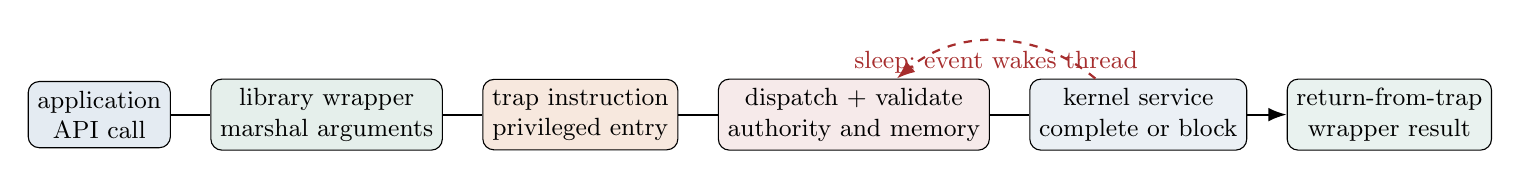
\begin{tikzpicture}[>=Latex,font=\small,node distance=5mm,every node/.style={align=center}]
    \node[draw,rounded corners,fill=osblue!12] (api) {application\\API call};
    \node[draw,rounded corners,fill=osgreen!12,right=of api] (wrap) {library wrapper\\marshal arguments};
    \node[draw,rounded corners,fill=osorange!15,right=of wrap] (entry) {trap instruction\\privileged entry};
    \node[draw,rounded corners,fill=osred!10,right=of entry] (valid) {dispatch + validate\\authority and memory};
    \node[draw,rounded corners,fill=osblue!9,right=of valid] (work) {kernel service\\complete or block};
    \node[draw,rounded corners,fill=osgreen!10,right=of work] (ret) {return-from-trap\\wrapper result};
    \draw[->,thick] (api)--(wrap)--(entry)--(valid)--(work)--(ret);
    \draw[->,thick,dashed,osred,bend right=40] (work) to node[below]{sleep; event wakes thread}(valid);
  \end{tikzpicture}}
  \vspace{0.5em}
  \begin{columns}[T,onlytextwidth]
    \column{0.48\textwidth}
      \begin{itemize}
        \item Entry changes privilege within the \emph{same thread}.
        \item Blocking makes the thread non-runnable; the scheduler may run another thread.
      \end{itemize}
    \column{0.48\textwidth}
      \begin{itemize}
        \item Errors are ordinary results at the ABI; libc commonly maps a negative error convention to \code{-1} and \code{errno}.
        \item Return may be partial even without an error.
      \end{itemize}
  \end{columns}
  \note{A syscall entry is a mode switch, not automatically a process context switch. If the call completes immediately, the thread can return directly. If it blocks, a scheduling decision follows. Linux kernel-internal error conventions and userspace libc errno conventions should not be presented as universal across OSes.}
\end{frame}

\begin{frame}{Example ABI: Linux on x86-64}
  \begin{columns}[T,onlytextwidth]
    \column{0.56\textwidth}
      \begin{block}{Conceptual register convention}
        \begin{tabular}{@{}ll@{}}
          syscall number & \code{rax} \\
          arguments 1--6 & \code{rdi, rsi, rdx, r10, r8, r9} \\
          result & \code{rax} \\
          entry instruction & \code{syscall} \\
        \end{tabular}
      \end{block}
      CPU/kernel entry code also handles:
      \begin{itemize}
        \item transition to a protected kernel execution context;
        \item saving enough architectural state to resume;
        \item speculation/entry mitigations required by the platform;
        \item dispatch through the syscall table or equivalent mechanism.
      \end{itemize}
    \column{0.40\textwidth}
      \begin{alertblock}{Architecture-specific}
        AArch64 uses different registers and \code{svc}; 32-bit x86 and compatibility ABIs differ again. Never hard-code an ABI when a maintained library interface suffices.
      \end{alertblock}
      \begin{tcolorbox}[title=Why wrappers matter]
        They handle calling conventions, symbol/version compatibility, cancellation points, \code{errno}, and alternate fast paths.
      \end{tcolorbox}
  \end{columns}
  \note{On x86-64, syscall also clobbers rcx and r11. The slide intentionally omits entry-stub details that vary with kernel configuration and mitigations. Students writing raw assembly should consult the exact ABI documentation rather than extrapolate from a C prototype.}
\end{frame}

\begin{frame}{Validation: user pointers are untrusted capabilities to memory}
  \begin{columns}[T,onlytextwidth]
    \column{0.52\textwidth}
      Kernel code must treat every argument as adversarial:
      \begin{itemize}
        \item syscall number, flags, lengths, alignment, and overflow;
        \item descriptor/handle validity and requested rights;
        \item pointer range, access direction, and faultability;
        \item object lifetime, concurrent mutation, and namespace context;
        \item policy checks from credentials, capabilities, ACLs, or labels.
      \end{itemize}
    \column{0.45\textwidth}
      \begin{tcolorbox}[title=Copying is a semantic boundary]
        Kernels use guarded primitives such as conceptual \code{copy\_from\_user}. A range check alone is insufficient: the page can fault, mappings can change, and user data can be modified concurrently.
      \end{tcolorbox}
      \begin{alertblock}{TOCTOU}
        Do not validate mutable user memory and later trust it unchanged. Copy once into kernel-owned memory or use a protocol that pins/locks and defines concurrency.
      \end{alertblock}
  \end{columns}
  \note{Pointer validation is not merely checking that an address is below a boundary. Access may fault and must be recoverable. Nested pointers require careful staged copying. Pinning pages solves some lifetime problems but creates resource-exhaustion and migration issues.}
\end{frame}

\begin{frame}{File descriptors: names for kernel objects and authority}
  \small
  \begin{columns}[T,onlytextwidth]
    \column{0.49\textwidth}
      \centering
      \resizebox{\linewidth}{!}{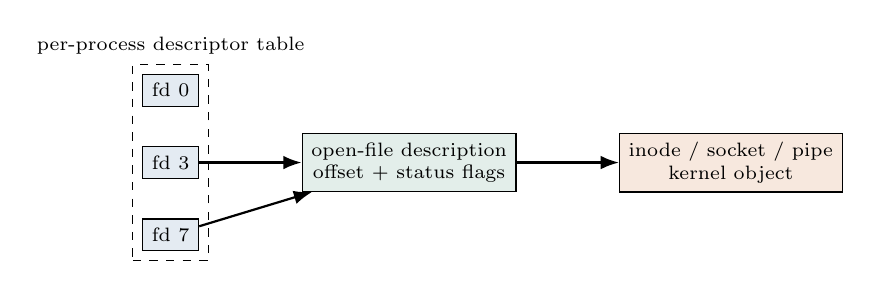
\begin{tikzpicture}[>=Latex,font=\scriptsize,node distance=5mm,every node/.style={align=center}]
        \node[draw,fill=osblue!12] (fd0) {fd 0};
        \node[draw,fill=osblue!12,below=of fd0] (fd3) {fd 3};
        \node[draw,fill=osblue!12,below=of fd3] (fd7) {fd 7};
        \node[draw,fill=osgreen!13,right=1.3cm of fd3] (ofd) {open-file description\\offset + status flags};
        \node[draw,fill=osorange!15,right=1.3cm of ofd] (obj) {inode / socket / pipe\\kernel object};
        \draw[->,thick] (fd3)--(ofd);
        \draw[->,thick] (fd7)--(ofd);
        \draw[->,thick] (ofd)--(obj);
        \node[draw,dashed,fit=(fd0)(fd3)(fd7),label=above:{per-process descriptor table}] {};
      \end{tikzpicture}}
    \column{0.48\textwidth}
      \begin{itemize}
        \item A descriptor indexes a process table; it is not the file itself.
        \item \code{dup()} creates another descriptor referencing the same open-file description, including file offset.
        \item \code{fork()} inherits descriptors; \code{execve()} preserves them unless close-on-exec is set.
        \item Descriptor possession conveys authority to invoke allowed operations on the referenced object.
      \end{itemize}
      \begin{alertblock}{Common failure}
        Leaked descriptors can keep files, pipes, sockets, mounts, or privileges alive and can cross an \code{execve()} boundary unexpectedly.
      \end{alertblock}
  \end{columns}
\end{frame}

\begin{frame}{Blocking, interruption, restart, and partial completion}
  \small
  \begin{tabularx}{\textwidth}{@{}lX@{}}
    \toprule
    \textbf{Outcome} & \textbf{Meaning and obligation} \\
    \midrule
    success & requested operation completed; returned count/value still matters \\
    partial success & some bytes/items completed; advance buffers and retry only if semantics permit \\
    \code{EINTR} & an interrupting signal was handled before completion; restart behavior depends on call, flags, and signal setup \\
    \code{EAGAIN} & nonblocking operation cannot progress now; wait for readiness or retry under a policy \\
    short read / EOF & fewer bytes can be valid; zero from a regular stream read commonly indicates EOF \\
    blocking & thread sleeps on a wait queue until state changes, timeout expires, or cancellation/signal occurs \\
    \bottomrule
  \end{tabularx}
  \begin{tcolorbox}[title=Robustness rule,colback=osgreen!5,colframe=osgreen!65]
    ``No error'' does not imply ``all requested work completed.'' Design loops around the API's precise progress and cancellation contract.
  \end{tcolorbox}
\end{frame}

% =============================================================================
\section{Robust Unix Programming Patterns}
% =============================================================================

\begin{frame}[fragile]{Robust writes: handle progress and interruption}
\begin{lstlisting}[language=C]
#include <errno.h>
#include <stddef.h>
#include <unistd.h>

int write_all(int fd, const void *buf, size_t len) {
    const unsigned char *p = buf;
    while (len != 0) {
        ssize_t n = write(fd, p, len);
        if (n > 0) { p += (size_t)n; len -= (size_t)n; continue; }
        if (n < 0 && errno == EINTR) continue;
        return -1;                 // includes EPIPE, EAGAIN, device error
    }
    return 0;
}
\end{lstlisting}
  \begin{columns}[T,onlytextwidth]
    \column{0.48\textwidth}
      \begin{itemize}
        \item \code{ssize\_t}, not \code{int}, represents byte counts/errors.
        \item A successful \code{write()} can be short.
      \end{itemize}
    \column{0.48\textwidth}
      \begin{itemize}
        \item Nonblocking descriptors need readiness integration, not a busy retry loop.
        \item Broken pipes involve \code{SIGPIPE}/\code{EPIPE} policy.
      \end{itemize}
  \end{columns}
  \note{This helper is suitable for blocking descriptors when the policy is to finish or fail. It deliberately does not spin on EAGAIN. Discuss why retrying an operation after partial progress can be unsafe for message- or transaction-oriented protocols unless the caller tracks framing.}
\end{frame}

\begin{frame}[fragile]{Safe file copy: descriptors, errors, and cleanup}
\begin{lstlisting}[language=C]
int in = open(src, O_RDONLY | O_CLOEXEC);
if (in < 0) fail("open source");
int out = open(dst, O_WRONLY | O_CREAT | O_TRUNC | O_CLOEXEC, 0644);
if (out < 0) { int e = errno; close(in); errno = e; fail("open dst"); }

unsigned char buf[64 * 1024];
for (;;) {
    ssize_t n = read(in, buf, sizeof buf);
    if (n > 0) { if (write_all(out, buf, (size_t)n) < 0) fail("write"); }
    else if (n == 0) break;
    else if (errno != EINTR) fail("read");
}
if (close(out) < 0) fail("close output"); // delayed write error possible
if (close(in) < 0) fail("close input");
\end{lstlisting}
  \smallnote{For security-sensitive replacement, also reason about symlink races, file mode/ownership, atomic rename, durability, sparse files, metadata, and whether source and destination name the same object.}
\end{frame}

\begin{frame}[fragile]{\code{fork()}--\code{execve()}--\code{waitpid()}: corrected pattern}
\begin{lstlisting}[language=C]
pid_t pid = fork();
if (pid < 0) fail("fork");
if (pid == 0) {
    execlp("ls", "ls", "-l", (char *)NULL);
    static const char msg[] = "exec failed\n";
    (void)write(STDERR_FILENO, msg, sizeof msg - 1);
    _exit(127);
}

int status;
while (waitpid(pid, &status, 0) < 0) {
    if (errno != EINTR) fail("waitpid");
}
\end{lstlisting}
  \begin{itemize}
    \item \code{fork()} returns twice; \code{exec} replaces the child's program image and returns only on failure.
    \item Use \code{\_exit()} in the failed child path to avoid flushing inherited stdio buffers or running parent cleanup handlers.
    \item In a multithreaded process, only async-signal-safe operations are permitted between \code{fork()} and \code{exec}; \code{posix\_spawn()} is often safer.
  \end{itemize}
  \note{Do not state categorically that Linux fork is implemented by a public clone syscall; libc and kernel implementation paths evolve. The semantic contract is more important: logically duplicated process state with copy-on-write memory in common implementations.}
\end{frame}

\begin{frame}[fragile]{Pipe discipline: EOF depends on closing every writer}
  \begin{columns}[T,onlytextwidth]
    \column{0.52\textwidth}
\begin{lstlisting}[language=C]
int p[2];
if (pipe2(p, O_CLOEXEC) < 0) fail("pipe2");
pid_t pid = fork();
if (pid == 0) {
    close(p[1]);
    if (dup2(p[0], STDIN_FILENO) < 0) _exit(126);
    close(p[0]);
    execlp("wc", "wc", "-w", (char *)NULL);
    _exit(127);
}
close(p[0]);
if (write_all(p[1], "hello world\n", 12) < 0)
    fail("pipe write");
close(p[1]);                    // lets wc observe EOF
\end{lstlisting}
    \column{0.44\textwidth}
      \begin{itemize}
        \item A pipe is a byte stream with bounded kernel buffering.
        \item Reads block while the buffer is empty and at least one write end remains open.
        \item The reader sees EOF only after the buffer drains and \emph{all} write references close.
        \item Writes up to \code{PIPE\_BUF} have defined atomicity properties; larger writes can interleave.
      \end{itemize}
  \end{columns}
\end{frame}

\begin{frame}{Memory mapping is an interface to the page cache and VM}
  \begin{columns}[T,onlytextwidth]
    \column{0.48\textwidth}
      \begin{itemize}
        \item \code{mmap()} creates a mapping; it does not necessarily read file data immediately.
        \item First access can fault pages into memory.
        \item \code{MAP\_PRIVATE} writes use copy-on-write; \code{MAP\_SHARED} can modify the shared mapping/file.
        \item Access beyond the valid backing object can raise a fault such as \code{SIGBUS}.
      \end{itemize}
    \column{0.48\textwidth}
      \begin{alertblock}{Unsafe original pattern}
        Mapping and writing a fixed 100 bytes without checking file length, \code{MAP\_FAILED}, or short output can access invalid pages or emit unrelated data.
      \end{alertblock}
      \begin{tcolorbox}[title=Use when]
        Random access, shared-memory protocols, or avoiding explicit copies helps enough to justify page-fault and coherence complexity.
      \end{tcolorbox}
  \end{columns}
\end{frame}

\begin{frame}{Signals: asynchronous delivery changes control flow}
  \begin{columns}[T,onlytextwidth]
    \column{0.51\textwidth}
      Correct design normally uses:
      \begin{itemize}
        \item \code{sigaction()}, not legacy \code{signal()}, for defined control;
        \item blocked signal masks while installing handlers and updating shared state;
        \item only async-signal-safe functions inside handlers;
        \item \code{sigsuspend()}, \code{sigwaitinfo()}, \code{signalfd()}, or an event loop to avoid check-then-sleep races.
      \end{itemize}
    \column{0.45\textwidth}
      \begin{alertblock}{Classic lost wakeup}
        ``Check flag; then call \code{pause()}'' races with a signal arriving between the check and sleep. Atomically replace the signal mask while waiting.
      \end{alertblock}
      \begin{tcolorbox}[title=Handler rule]
        Do minimal work: record state using an appropriate atomic/signal-safe mechanism or write to a self-pipe, then handle complexity in normal control flow.
      \end{tcolorbox}
  \end{columns}
\end{frame}

% =============================================================================
\section{Performance, Observability, and Security}
% =============================================================================

\begin{frame}{Where syscall cost comes from}
  \begin{columns}[T,onlytextwidth]
    \column{0.50\textwidth}
      \textbf{Direct cost}
      \begin{itemize}
        \item wrapper and trap/return instructions;
        \item entry bookkeeping and mitigations;
        \item dispatch, validation, copying, accounting;
        \item locks and kernel data-structure traversal.
      \end{itemize}
    \column{0.47\textwidth}
      \textbf{Indirect/dominant cost}
      \begin{itemize}
        \item cache/TLB disruption;
        \item blocking and scheduling latency;
        \item page faults or device/network queues;
        \item contention, write-back, and remote services.
      \end{itemize}
  \end{columns}
  \begin{tcolorbox}[title=Simple cost model]
    For $N$ operations of payload $B$, a useful first model is
    \[
      T \approx N\,t_{\text{fixed}} + NB\,t_{\text{per-byte}} + T_{\text{queueing}} + T_{\text{device}}.
    \]
    Batching reduces the fixed term but can increase waiting latency and memory footprint.
  \end{tcolorbox}
  \note{The equation is a decomposition, not a universal predictive law. Ask which term dominates for getpid, a cached 4 KiB read, and a disk miss. Benchmark warm and cold cases separately and report distributions rather than one context-free nanosecond number.}
\end{frame}

\begin{frame}{Avoiding or amortizing crossings}
  \scriptsize
  \begin{tabularx}{\textwidth}{@{}lXX@{}}
    \toprule
    \textbf{Technique} & \textbf{Mechanism} & \textbf{Trade-off} \\
    \midrule
    buffering/batching & more work per call & added latency, memory, failure granularity \\
    \code{readv}/\code{writev} & scatter/gather buffers & descriptor/vector limits; still copies in many paths \\
    memory mapping & page-based sharing/access & page faults, coherence, invalidation complexity \\
    vDSO & kernel-published data + user code & only suitable for carefully designed read-mostly services \\
    asynchronous queues & submit/completion rings, e.g., \code{io\_uring} & lifecycle, cancellation, pinning, security complexity \\
    user-space networking/storage & map queues and poll devices & dedicates cores; shifts protection and driver burden \\
    \bottomrule
  \end{tabularx}
  \begin{alertblock}{Optimization boundary}
    Removing syscall crossings does not remove the need for authorization, isolation, resource accounting, or synchronization; it relocates their mechanisms.
  \end{alertblock}
\end{frame}

\begin{frame}{Observability: choose the tool for the question}
  \begin{columns}[T,onlytextwidth]
    \column{0.50\textwidth}
      \begin{itemize}
        \item \code{strace}: syscall names, arguments, results, timing; perturbation can be substantial.
        \item \code{perf}: hardware/software counters, sampling, scheduling and fault statistics.
        \item eBPF tracing: programmable kernel probes and aggregation with safety constraints.
        \item application tracing: semantic spans and request IDs unavailable to the kernel alone.
      \end{itemize}
    \column{0.47\textwidth}
      \begin{tcolorbox}[title=Do not infer too much]
        A trace line shows the interface event, not necessarily physical I/O. A \code{read()} may hit the page cache; work may have occurred earlier through read-ahead or later through write-back.
      \end{tcolorbox}
      \begin{block}{Measurement protocol}
        State workload, kernel/hardware, cache state, concurrency, tracing overhead, metric definition, and latency distribution.
      \end{block}
  \end{columns}
\end{frame}

\begin{frame}{System-call attack surface and mediation}
  \begin{columns}[T,onlytextwidth]
    \column{0.52\textwidth}
      Defensive mechanisms include:
      \begin{itemize}
        \item least-privilege credentials and Linux capabilities;
        \item seccomp filters restricting syscall numbers/arguments;
        \item namespaces, cgroups, MAC/LSM policies, and sandbox brokers;
        \item descriptor passing instead of ambient pathname authority;
        \item memory-safe implementations, fuzzing, and formal verification.
      \end{itemize}
    \column{0.44\textwidth}
      \begin{alertblock}{Filtering is not authorization}
        Allowing \code{read()} says nothing about which descriptors may be read. Conversely, blocking one syscall may not remove equivalent authority through another path.
      \end{alertblock}
      \begin{tcolorbox}[title=Design objective]
        Reduce reachable kernel code and ambient authority while preserving the minimal operations the workload needs.
      \end{tcolorbox}
  \end{columns}
  \note{seccomp is an attack-surface reduction mechanism, not a complete sandbox. It does not virtualize namespaces, constrain resource consumption, or express all object-level policy. Descriptor-oriented designs can make authority explicit and delegable.}
\end{frame}

% =============================================================================
\section{Operating-System Structures}
% =============================================================================

\begin{frame}{Architecture is placement plus communication}
  Instead of memorizing labels, characterize a design along these dimensions:
  \begin{columns}[T,onlytextwidth]
    \column{0.49\textwidth}
      \begin{itemize}
        \item Which services execute privileged?
        \item What belongs to the trusted computing base?
        \item Are calls procedure calls, traps, messages, or shared-memory protocols?
        \item Which failures can be restarted or contained?
      \end{itemize}
    \column{0.48\textwidth}
      \begin{itemize}
        \item How are authority and names represented?
        \item Can components evolve independently?
        \item What state crosses protection domains?
        \item Which paths require verification or certification?
      \end{itemize}
  \end{columns}
  \begin{tcolorbox}[title=Mechanism--policy separation]
    Structure determines communication and trust boundaries. It does not by itself determine scheduling, caching, naming, or security policy.
  \end{tcolorbox}
\end{frame}

\begin{frame}{Monolithic but modular kernels}
  \small
  \begin{columns}[T,onlytextwidth]
    \column{0.48\textwidth}
      \centering
      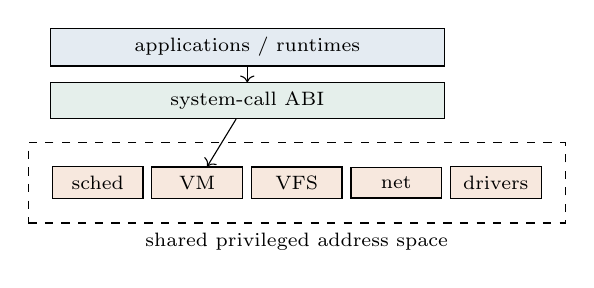
\begin{tikzpicture}[font=\scriptsize,node distance=2mm,every node/.style={align=center}]
        \node[draw,fill=osblue!12,minimum width=5cm] (apps) {applications / runtimes};
        \node[draw,fill=osgreen!12,minimum width=5cm,below=of apps] (abi) {system-call ABI};
        \node[draw,fill=osorange!15,minimum width=1.15cm,below=6mm of abi,xshift=-1.9cm] (sched) {sched};
        \node[draw,fill=osorange!15,minimum width=1.15cm,right=1mm of sched] (vm) {VM};
        \node[draw,fill=osorange!15,minimum width=1.15cm,right=1mm of vm] (vfs) {VFS};
        \node[draw,fill=osorange!15,minimum width=1.15cm,right=1mm of vfs] (net) {net};
        \node[draw,fill=osorange!15,minimum width=1.15cm,right=1mm of net] (drv) {drivers};
        \node[draw,dashed,fit=(sched)(vm)(vfs)(net)(drv),inner sep=3mm,label=below:{shared privileged address space}] {};
        \draw[->] (apps)--(abi);
        \draw[->] (abi)--(vm);
      \end{tikzpicture}
    \column{0.49\textwidth}
      \begin{itemize}
        \item Kernel subsystems communicate with direct calls and shared internal state.
        \item Loadable modules allow runtime extension but usually share kernel privilege and failure fate.
        \item Strengths: mature integration, low call overhead, efficient shared caches.
        \item Risks: large TCB/attack surface; memory corruption or driver faults can compromise the whole kernel.
      \end{itemize}
      \begin{block}{Examples}
        Linux and BSD are commonly described as monolithic, modular kernels---not ``hybrid monolithic.''
      \end{block}
  \end{columns}
  \note{Modularity is a software-organization property; isolation is a protection property. A loadable module can be well structured yet still execute with full kernel privilege. Modern Linux also moves many services to user space, so labels describe the privileged core rather than the entire operating environment.}
\end{frame}

\begin{frame}{Layering and information hiding}
  \small
  \begin{columns}[T,onlytextwidth]
    \column{0.44\textwidth}
      \centering
      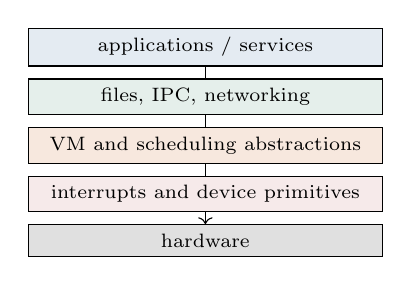
\begin{tikzpicture}[font=\scriptsize,node distance=1.5mm]
        \node[draw,fill=osblue!12,minimum width=4.5cm] (l4) {applications / services};
        \node[draw,fill=osgreen!12,minimum width=4.5cm,below=of l4] (l3) {files, IPC, networking};
        \node[draw,fill=osorange!15,minimum width=4.5cm,below=of l3] (l2) {VM and scheduling abstractions};
        \node[draw,fill=osred!10,minimum width=4.5cm,below=of l2] (l1) {interrupts and device primitives};
        \node[draw,fill=black!12,minimum width=4.5cm,below=of l1] (l0) {hardware};
        \draw[->] (l4)--(l3)--(l2)--(l1)--(l0);
      \end{tikzpicture}
    \column{0.52\textwidth}
      \begin{itemize}
        \item Each layer exposes an abstraction and hides lower-level representation.
        \item Benefits: local reasoning, replaceable implementations, test seams, reduced coupling.
        \item Costs: strict layering can force redundant conversions/copies or awkward dependency inversions.
        \item Real kernels often use \concept{layering with controlled bypasses}, not a perfectly linear stack.
      \end{itemize}
      \begin{tcolorbox}[title=Examples]
        VFS over multiple filesystems is a strong interface boundary; network stacks are layered conceptually but optimize across layers.
      \end{tcolorbox}
  \end{columns}
\end{frame}

\begin{frame}{Microkernel: minimal privileged mechanism}
  \centering
  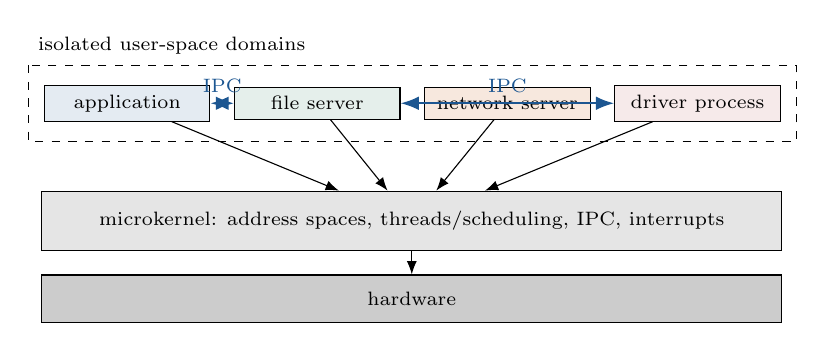
\begin{tikzpicture}[>=Latex,font=\scriptsize,node distance=3mm,every node/.style={align=center}]
    \node[draw,fill=osblue!12,minimum width=2.1cm] (app) {application};
    \node[draw,fill=osgreen!12,minimum width=2.1cm,right=of app] (fs) {file server};
    \node[draw,fill=osorange!15,minimum width=2.1cm,right=of fs] (net) {network server};
    \node[draw,fill=osred!10,minimum width=2.1cm,right=of net] (drv) {driver process};
    \node[draw,fill=black!10,minimum width=9.4cm,minimum height=.75cm,below=9mm of fs,xshift=1.2cm] (mk) {microkernel: address spaces, threads/scheduling, IPC, interrupts};
    \node[draw,fill=black!20,minimum width=9.4cm,minimum height=.6cm,below=of mk] (hw) {hardware};
    \draw[<->,thick,osblue] (app) -- node[above]{IPC} (fs);
    \draw[<->,thick,osblue] (fs) -- node[above]{IPC} (drv);
    \draw[->] (app)--(mk); \draw[->] (fs)--(mk); \draw[->] (net)--(mk); \draw[->] (drv)--(mk); \draw[->] (mk)--(hw);
    \draw[dashed] ($(app.north west)+(-.2,.25)$) rectangle ($(drv.south east)+(.2,-.25)$);
    \node[anchor=west] at ($(app.north west)+(-.2,.5)$) {isolated user-space domains};
  \end{tikzpicture}
  \begin{columns}[T,onlytextwidth]
    \column{0.49\textwidth}
      \textbf{Potential strengths}
      \begin{itemize}
        \item smaller privileged TCB;
        \item fault containment/restartable services;
        \item explicit authority and message interfaces.
      \end{itemize}
    \column{0.48\textwidth}
      \textbf{Design costs}
      \begin{itemize}
        \item IPC crossings, scheduling handoffs, data transfer;
        \item distributed state and recovery protocols;
        \item performance depends strongly on IPC design and workload.
      \end{itemize}
  \end{columns}
  \note{Avoid saying microkernels are inherently slow. Early designs exposed significant IPC overhead, while later kernels use optimized IPC, shared memory, batching, and careful scheduling. Fault isolation is only useful if protocols can recover and dependent state is reconstructible.}
\end{frame}

\begin{frame}{Fast IPC is more than copying bytes}
  For a client request to a user-space server, latency may include:
  \[
    T_{\text{IPC}} = T_{\text{entry}} + T_{\text{validation}} + T_{\text{handoff}}
      + T_{\text{data}} + T_{\text{cache/TLB}} + T_{\text{queue}}.
  \]
  \begin{columns}[T,onlytextwidth]
    \column{0.49\textwidth}
      Optimization techniques:
      \begin{itemize}
        \item register-based small messages;
        \item direct process handoff/donation;
        \item shared-memory data planes;
        \item batching and asynchronous completion;
        \item capability lookup integrated with IPC.
      \end{itemize}
    \column{0.47\textwidth}
      \begin{alertblock}{End-to-end caveat}
        Moving a driver into user space may add crossings but reduce recovery time, privileged code, and certification scope. Architecture evaluation must include failure and maintenance cost, not only steady-state throughput.
      \end{alertblock}
  \end{columns}
\end{frame}

\begin{frame}{Hybrid kernels: a descriptive family, not a theorem}
  \begin{columns}[T,onlytextwidth]
    \column{0.51\textwidth}
      Systems commonly called hybrid retain microkernel-inspired abstractions while executing substantial services in one privileged address space for pragmatic performance or compatibility.
      \begin{itemize}
        \item Windows NT: executive subsystems and kernel-mode components above an NT kernel/HAL foundation.
        \item XNU: Mach-derived primitives plus BSD and I/O Kit components in the kernel.
      \end{itemize}
    \column{0.45\textwidth}
      \begin{tcolorbox}[title=Do not overread the label]
        ``Hybrid'' does not guarantee the best of both worlds. Ask which components are actually isolated, how they communicate, and which faults remain kernel-fatal.
      \end{tcolorbox}
      \begin{block}{Comparison rule}
        Compare concrete paths and trust boundaries, not marketing categories.
      \end{block}
  \end{columns}
\end{frame}

\begin{frame}{Beyond the classical taxonomy}
  \small
  \begin{tabularx}{\textwidth}{@{}lXX@{}}
    \toprule
    \textbf{Design} & \textbf{Core idea} & \textbf{Trade-off} \\
    \midrule
    Exokernel & securely multiplex hardware; applications choose abstractions & flexibility and specialization versus complex library OSes \\
    Library OS & link OS services as application libraries over a host/hypervisor & per-application policy; duplicated state/services \\
    Unikernel & compile one application with minimal OS components into an image & small footprint and attack surface; debugging/compatibility challenges \\
    Multiserver OS & decompose services into isolated cooperating processes & restartability and least privilege; protocol/state complexity \\
    Type-safe / language OS & use language guarantees to constrain components & smaller bug classes; toolchain/runtime trust and unsafe boundaries \\
    Formally verified kernel & prove specified properties of the implementation & strong assurance within assumptions; specification/proof cost \\
    \bottomrule
  \end{tabularx}
  \smallnote{These approaches can be combined with hardware virtualization, containers, capabilities, and conventional kernels.}
\end{frame}

\begin{frame}{Trusted computing base and verification boundary}
  \begin{columns}[T,onlytextwidth]
    \column{0.50\textwidth}
      \concept{TCB}: components whose failure can violate the target security/correctness property.
      \begin{itemize}
        \item Smaller code size can help review and verification, but interface complexity matters too.
        \item Hardware, boot chain, compiler, firmware, DMA configuration, and privileged services may be in the effective TCB.
        \item A proof establishes a theorem about a model/specification under assumptions; it is not an all-purpose guarantee.
      \end{itemize}
    \column{0.46\textwidth}
      \begin{tcolorbox}[title=Example: seL4]
        seL4 demonstrates that strong machine-checked kernel properties are feasible. System-level assurance still requires correct user-space services, configurations, hardware assumptions, and refinement between models and deployment.
      \end{tcolorbox}
      \begin{alertblock}{Security lesson}
        Minimize both privileged implementation and ambient authority reachable through its interfaces.
      \end{alertblock}
  \end{columns}
  \note{Be careful not to imply that all seL4-based systems are fully verified end to end. Explain the difference among functional correctness, information-flow properties, binary verification, and availability. The exact verified configuration and assumptions matter.}
\end{frame}

\begin{frame}{Architecture comparison: replace rankings with questions}
  \scriptsize
  \begin{tabularx}{\textwidth}{@{}lXXXX@{}}
    \toprule
    & \textbf{Monolithic/modular} & \textbf{Microkernel} & \textbf{Hybrid} & \textbf{Library OS / unikernel} \\
    \midrule
    Privileged scope & broad kernel services & minimal mechanisms & broad, pragmatically arranged & host/hypervisor plus linked image \\
    Communication & direct calls/shared state & IPC/shared memory & both & local calls to linked services \\
    Fault containment & limited inside kernel & service-domain boundaries & path-dependent & VM/process boundary-dependent \\
    Specialization & configurable/general & replaceable servers & subsystem-specific & high per-application specialization \\
    Key cost & TCB and fault blast radius & IPC/recovery complexity & conceptual and implementation complexity & duplication, tooling, compatibility \\
    Best evidence & workload and fault tests & IPC plus recovery measurements & concrete component map & image/host threat and operations model \\
    \bottomrule
  \end{tabularx}
  \begin{tcolorbox}[title=Decision principle]
    Choose an architecture for a specified workload, failure model, threat model, certification target, and maintenance organization---not from a universal ``fastest'' or ``safest'' ranking.
  \end{tcolorbox}
\end{frame}

\begin{frame}{Case study matrix}
  \small
  \begin{tabularx}{\textwidth}{@{}lXXX@{}}
    \toprule
    \textbf{System} & \textbf{Structural emphasis} & \textbf{Useful lesson} & \textbf{Do not claim} \\
    \midrule
    Linux & monolithic, modular kernel; extensive user-space services & integration and performance with a large ecosystem & modules provide fault isolation \\
    Windows NT & hybrid family with object-based executive and subsystem history & compatibility and layered internal interfaces & all services are isolated microkernel servers \\
    XNU/macOS & Mach + BSD + I/O Kit in a privileged kernel & architectures accrete and combine lineages & the ``hybrid'' label predicts every path \\
    QNX & commercial microkernel with user-space services & fault containment and real-time deployment & microkernel alone guarantees deadlines \\
    seL4 & capability microkernel with formal verification results & explicit authority and proof-oriented design & the whole deployed system is automatically verified \\
    \bottomrule
  \end{tabularx}
\end{frame}

% =============================================================================
\section{Synthesis}
% =============================================================================

\begin{frame}{From application call to architecture choice}
  \centering
  \resizebox{.94\textwidth}{!}{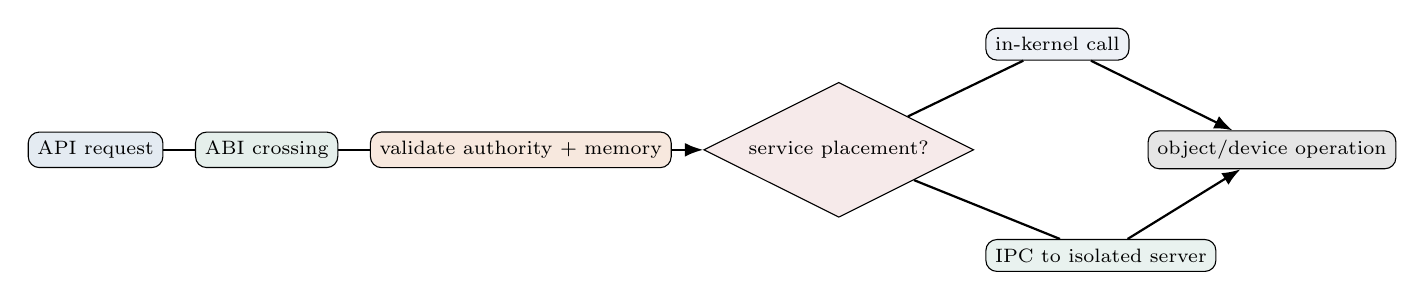
\begin{tikzpicture}[>=Latex,font=\scriptsize,node distance=4mm,every node/.style={align=center}]
    \node[draw,rounded corners,fill=osblue!12] (app) {API request};
    \node[draw,rounded corners,fill=osgreen!12,right=of app] (abi) {ABI crossing};
    \node[draw,rounded corners,fill=osorange!15,right=of abi] (auth) {validate authority + memory};
    \node[draw,diamond,aspect=2,fill=osred!10,right=of auth] (where) {service placement?};
    \node[draw,rounded corners,fill=osblue!8,above right=7mm and 10mm of where] (ink) {in-kernel call};
    \node[draw,rounded corners,fill=osgreen!10,below right=7mm and 10mm of where] (ipc) {IPC to isolated server};
    \node[draw,rounded corners,fill=black!10,right=2.2cm of where] (obj) {object/device operation};
    \draw[->,thick] (app)--(abi)--(auth)--(where);
    \draw[->,thick] (where)--(ink)--(obj);
    \draw[->,thick] (where)--(ipc)--(obj);
  \end{tikzpicture}}
  \begin{tcolorbox}[title=The recurring trade-off]
    Direct calls and shared state minimize crossing overhead but enlarge trust and failure domains. Isolated servers make authority and failure boundaries explicit but require IPC, state partitioning, and recovery protocols.
  \end{tcolorbox}
\end{frame}

\begin{frame}{Misconceptions corrected}
  \small
  \begin{tabularx}{\textwidth}{@{}X@{\quad$\Rightarrow$\quad}X@{}}
    \toprule
    \textbf{Misconception} & \textbf{Precise statement} \\
    \midrule
    Every libc call is a syscall. & Libraries may compute, buffer, or invoke different/multiple syscalls. \\
    A syscall always context-switches. & It changes privilege; scheduling another thread is conditional. \\
    Successful \code{read}/\code{write} transfers all bytes. & Short counts are valid and must drive control flow. \\
    Linux \code{fork()} literally copies all memory. & The semantics are copying; implementations commonly use COW. \\
    Microkernels are necessarily slow. & Performance depends on IPC, workload, batching, caches, and service design. \\
    Modules isolate kernel failures. & Modules improve extensibility but usually share kernel privilege. \\
    Hybrid means optimal compromise. & It is a descriptive label; inspect concrete placement and boundaries. \\
    seccomp is a complete sandbox. & It restricts syscall reachability, not all object authority or resource use. \\
    \bottomrule
  \end{tabularx}
\end{frame}

\begin{frame}{Key takeaways}
  \begin{itemize}
    \item The API, library, ABI, and kernel object interface are distinct contracts.
    \item Syscall correctness depends on validation, explicit authority, safe copying, progress semantics, and descriptor lifetime.
    \item Performance is end-to-end: crossings matter, but queueing, faults, copying, caches, and devices often dominate.
    \item Kernel structure determines trust, communication, and failure boundaries; it does not automatically determine policy quality.
    \item Robust evaluation combines steady-state benchmarks, tail latency, failure injection, attack-surface analysis, and maintenance cost.
  \end{itemize}
  \begin{tcolorbox}[title=Transfer question,colback=osgreen!5,colframe=osgreen!65]
    For any OS service, identify the promised abstraction, representation of authority, protection crossings, blocking points, recoverable failures, and measurement plan.
  \end{tcolorbox}
\end{frame}

\begin{frame}{Laboratory: trace and explain a file copy}
  \begin{enumerate}
    \item Compile a correct file-copy program with warnings and sanitizers enabled.
    \item Trace it using \code{strace -f}; identify wrapper-visible calls, return counts, and descriptor lifetime.
    \item Compare cold-cache and warm-cache runs using timing and \code{perf stat}.
    \item Reduce syscall count using a larger buffer or vectored I/O; explain whether elapsed time changes.
    \item Inject failures: missing file, permission denial, full filesystem, broken pipe, and signal interruption.
  \end{enumerate}
  \begin{alertblock}{Report requirement}
    Distinguish observations from inferences. A syscall trace alone does not prove physical device access, durability, or a context switch.
  \end{alertblock}
\end{frame}

\begin{frame}{Next week: process and thread management}
  \begin{itemize}
    \item process/thread representation and lifecycle;
    \item creation, execution, waiting, signals, and termination;
    \item scheduling queues, policies, and multicore load balancing;
    \item context-switch state and indirect cache/TLB costs;
    \item hands-on process trees and scheduling observation.
  \end{itemize}
  \begin{tcolorbox}[title=Preparation]
    Run \code{ps -ef --forest}, inspect \code{/proc/<pid>/status} and \code{/proc/<pid>/fd}, then predict which attributes survive \code{fork()} and \code{execve()}.
  \end{tcolorbox}
\end{frame}

% =============================================================================
\appendix
\section{Appendix}
% =============================================================================

\begin{frame}{Knowledge check: interfaces}
  \begin{enumerate}
    \item Can \code{gettimeofday()} complete without entering kernel mode? Explain.
    \item Why can libc \code{open()} appear as \code{openat()} in a Linux trace?
    \item A blocking \code{read()} returns \code{-1/EINTR}. Under what conditions is retry appropriate?
    \item Why is ``validate pointer, then dereference later'' vulnerable to TOCTOU?
    \item Two descriptors created by \code{dup()} read from a regular file. Do they share an offset?
    \item Why can a pipe reader wait forever even after the intended writer closes its descriptor?
  \end{enumerate}
  \note{Answers: (1) yes, via a vDSO fast path. (2) libc may implement the API through another compatible syscall. (3) when no disallowed partial effect occurred and application cancellation semantics permit retry. (4) user mappings/data can change between check and use. (5) yes, they reference one open-file description. (6) another process or leaked descriptor still holds a write end.}
\end{frame}

\begin{frame}{Knowledge check: structure}
  \begin{enumerate}
    \item Why does a loadable module improve modularity without necessarily improving fault isolation?
    \item Name two costs beyond byte copying in a user-space server IPC path.
    \item When might a user-space driver outperform its fault-isolation cost?
    \item What belongs in the effective TCB of a verified-kernel deployment besides the kernel proof?
    \item Why is ``microkernel versus monolithic'' insufficient to choose an automotive OS?
  \end{enumerate}
  \begin{tcolorbox}[title=Discussion extension]
    Specify a workload and threat model, then draw the smallest protection-domain decomposition that meets latency, recovery, and certification goals.
  \end{tcolorbox}
\end{frame}

\begin{frame}{Exercise: design a syscall-safe record API}
  A user supplies a pointer to an array of variable-length records and asks the kernel to validate and store them atomically.
  \begin{enumerate}
    \item Identify integer-overflow, nested-pointer, fault, and TOCTOU risks.
    \item Propose a bounded wire format with explicit total length and offsets.
    \item Decide when copying, validation, allocation, authorization, and commit occur.
    \item Define partial-failure, cancellation, retry, and idempotency semantics.
    \item Explain how fuzzing and property-based tests would target the interface.
  \end{enumerate}
\end{frame}

\begin{frame}{Exercise: architecture for a safety controller}
  Requirements: bounded control-loop latency, restartable network stack, minimal certified code, device isolation, and field-updatable telemetry.
  \begin{enumerate}
    \item Place scheduler, interrupt handling, drivers, filesystems, networking, and update service into protection domains.
    \item Draw IPC and shared-memory paths.
    \item State the authority held by each component.
    \item Bound blocking and recovery time after a driver crash.
    \item Compare the proposal with a modular monolithic design.
  \end{enumerate}
\end{frame}

\begin{frame}[fragile]{Raw syscall demonstration: for ABI study only}
\begin{lstlisting}[language=C]
#include <sys/syscall.h>
#include <unistd.h>

long result = syscall(SYS_write, STDOUT_FILENO, "hello\n", 6);
\end{lstlisting}
  \begin{itemize}
    \item \code{syscall()} is itself a libc helper for issuing a syscall by number; it is not inline assembly here.
    \item It remains nonportable across OSes and sometimes architectures, and it can bypass wrapper features.
    \item Use it when studying or accessing a deliberately unsupported raw interface---not as a default replacement for maintained APIs.
  \end{itemize}
\end{frame}

\begin{frame}{Further study}
  \begin{itemize}
    \item ABI design: compatibility syscalls, structure versioning, feature negotiation.
    \item High-performance interfaces: shared rings, zero-copy, polling, userspace drivers.
    \item Security: capability systems, syscall brokers, seccomp, confused deputies.
    \item Microkernels: IPC design, multiserver recovery, scheduling-context donation.
    \item Assurance: refinement proofs, verified compilation, information flow, WCET analysis.
    \item Architecture: exokernels, library OSes, unikernels, confidential VMs.
  \end{itemize}
  \begin{center}
    \Large Questions?
  \end{center}
\end{frame}

\end{document}

